\section{\label{III-C-3}Des résultats à la hauteur des données initiales}
\titreEntete{Des résultats à la hauteur des données initiales}

%intro
Les résultats de l'automatisation d'un processus de traitement de données dépend entièrement de la qualité des données initiales. Les difficultés propres aux différences de structures entre les jeux de données ou aux différences de graphie, additionnées à celles posées par la volonté d'avoir des alignements fiables et sans doublons, sont autant de facteurs qui réduisent l'efficacité de l'alignement automatique de deux référentiels.\\

Dans le cas de l'alignement des référentiels de personnes de la \ac{dj} et de la \ac{ddcol}, les résultats reflètent les difficultés rencontrées, tant dans les quantités de résultats que dans les indices de confiance attribués. Cette hétérogénéité des résultats conduit à la nécessité d'une supervision humaine des alignements réalisés et non réalisés.

\subsection{\label{III-C-3-a}Des résultats hétérogènes reflétant les multiples difficultés}
\titreEntete{Des résultats hétérogènes}

Environ soixante pour cent des matricules de personnes de la \ac{dj} ont trouvé leur équivalent dans la \ac{ddcol}. Ce résultat, bien que faible, reflète les difficultés rencontrées, ainsi que la spécificité des usages de chaque référentiel. En effet, la \ac{dj} utilise les personnes pour leur verser des droits, ce qui signifie alors que ces personnes ne sont pas spécialement des acteurs des documents conservés à la \ac{ddcol} pour lesquels le référentiel des personnes physiques a été créé. Il est par conséquent normal de ne pas pouvoir aligner tous les matricules de la \ac{dj} avec la \ac{ddcol}, cette dernière n'ayant pas besoin de conserver les ayants-droits de chaque personne du référentiel.

\begin{figure}[!h]
	\centering
	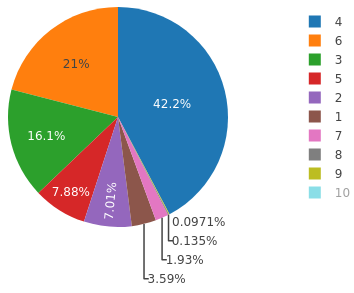
\includegraphics[width=8cm]{images/indices.png}
	\caption{Répartition des indices de confiance après les alignements entre les rééfrentiels de personnes de la \ac{dj} et de la \ac{ddcol}}
	\label{indices}
\end{figure}

La répartition des indices de confiance (\reference{indices}) reflète quant à elle à la fois la qualité des données initiales, ainsi que le processus d'alignement en lui-même. En effet, les différences de niveaux de précision dans les jeux de données initiaux conduisent à l'impossibilité d'utiliser certains points de comparaison, ce qui réduit l'indice de confiance: ces différences peuvent être une absence de données d'un côté de l'alignement, ou bien une divergence de graphie ou de structure qui n'a pas pu être corrigée lors du traitement préalable des données. Ainsi, l'indice \textit{4} est celui le plus présent en raison du faible nombre de points de comparaison qui le permettent: le nom, le prénom ainsi que la date ou une fonction suffisent à attribuer cet indice.\\

De plus, l'enchaînement des étapes entraîne également une diminution des indices de confiance: les étapes considérées comme prioritaires sont aussi celles qui utilisent les points de comparaison à la plus forte valeur. Ainsi, les indices de confiance attribués dans les alignements sont globalement inférieurs à cinq, et peu peuvent être considérés comme fiables quand l'indice est supérieur à cinq ou six.

\subsection{\label{III-C-3-b}Une supervision humaine nécessaire}
\titreEntete{Une supervision humaine nécessaire}

L'incertitude entourant la majorité des alignements conduit, comme cela est le cas pour le catalogage après la génération automatique de données, à utiliser une supervision humain. En effet, seule l'expertise et la réflexion d'un agent humain peut, ou non, confirmer les alignements produits. Seulement, cet agent humain va se heurter également à certaines problématiques posées dans l'automatisation: l'absence d'informations dans un matricule de la \ac{dj} ou dans un concept du \ldd ne permettra pas d'affirmer si les deux personnes alignées automatiquement sont réellement identiques et peuvent être associées.\\

Outre ce rejet ou cette acceptation des alignements réalisés automatiquement, la supervision humaine doit pouvoir modifier ce qui lui est proposé, ou bien pouvoir créer de nouveaux alignements. En effet, les jointures effectuées dans Talend\footnote{Elles sont au nombre de onze.} ne prennent pas en compte toutes les possibilités des deux jeux de données\footnote{Il existe quarante-deux (sept attributs sont disponibles dans la \ac{dj}, et six dans la \ac{ddcol}) jointures de stricte égalité possibles.} pour des raisons de fiabilité de ces possibilités dans le processus d'alignement. L'agent humain est seul capable de rechercher dans les données de la \ac{ddcol} un concept selon des critères que l'intelligence humaine offre: ils peuvent être l'inversion de deux lettres suite à une coquille dans la graphie, la francisation ou la traduction d'un terme étranger, l'inversion de deux prénoms, la connaissance d'un autre pseudonyme de la personne qui n'est pas spécifié dans les données de la \ac{dj}, \dots

%conlu
\bigskip
\bigskip
L'action humaine est toujours nécessaire, même avec un processus automatique d'alignement entre des données. Cette action est essentielle pour obtenir des données cohérentes et fiables dans un nouveau modèle de données. En effet, ces données étaient initialement cohérentes et sûres dans leurs bases de données respectives: elles doivent retrouver cette cohérence et cette fiabilité, même après un traitement automatique. Pour cela, la supervision humaine est nécessaire pour s'en assurer et proposer le cas échéant des solutions. 